\section{Analisis}

\begin{comment}
	Los archivos build.ninja los utiliza el ninja como si fuera el Makefile.
	Los archivos BUILD.gn los usa gn [gen] como si fuera el Makefile.
	
\end{comment}


\subsection{Construcción del sistema}
	Cada directorio relacionado con la construcción contiene un archivo \texttt{BUILD.gn} o algún archivo de inclusión \texttt{.gni} y gracias al funcionamiento, descrito en la \autoref{ssec:gn}, se construye \texttt{OpuntiaOS} de manera ordenada.

	
	
	El archivo \texttt{gn\_gen.sh} es el encargado de generar los archivos necesarios para comenzar la construcción del sistema dentro del directorio \texttt{out}, esto gracias a \texttt{GN}, ejecutándose como se observa en la \autoref{fig:buildArm} y \autoref{fig:buildx86}.
	
	
	
	La primera ejecución relevante está en la línea:
	\begin{center}
		\ttfamily
		gn gen \$OUTDIR --args=\$GNARGS,
	\end{center}
	
	donde \texttt{OUTDIR} es \texttt{out} y \texttt{GNARGS} es, en el caso de la \autoref{fig:buildArm} y \autoref{fig:buildx86}, la arquitectura que se va a construir, entonces toma el valor \texttt{target\_arch=''arm''} o \texttt{target\_arch=''x86''}, según corresponda.
	
	
	
	Este argumento es transmitido a través de todos los archivos \texttt{BUILD.gn} de los diferentes directorios, principalmente se lee esta condición en los archivos de construcción \texttt{build/boot/BUILD.gn} y \texttt{build/config/BUILDCONFIG.gn}, así como en los archivos de inclusión \texttt{toolchains/COMPILERS.gni} y \\ \texttt{build/userland/USERLAND\_FLAGS.gni}.
	
	\begin{figure}[ht]
		\centering
		\subfloat[\texttt{ARM}]{
			\includegraphics[scale=0.3]{outPrebuild_ARM.png}
		}
		\hspace*{0.3cm}
		\subfloat[\texttt{x86}]{
			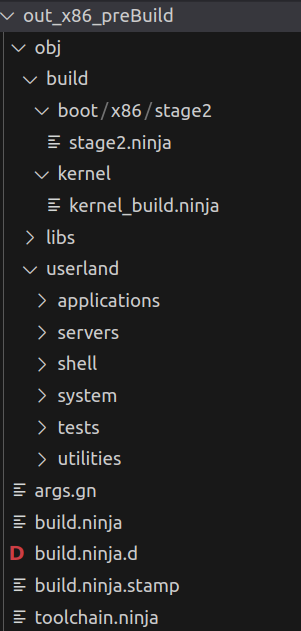
\includegraphics[scale=0.3]{outPrebuild_x86.png}
		}
		\caption{
			Árbol de carpetas del directorio \texttt{obj} creado previo a
			la construcción del sistema.
			\label{fig:outPrebuild}
		}
	\end{figure}

	
	\clearpage
	En este punto se genera un directorio que posteriormente es eliminado y contiene las definiciones \texttt{ninja} para la construcción de \textit{scripts} como \texttt{all.sh}, \texttt{build.sh}, \texttt{sync.sh} y \texttt{run.sh}, así como la compilación de los archivos de \textit{boot}, mismos cuyo código se encuentra en los directorios mostrados en la \autoref{fig:implBootloader}.
	
	
	
	La estructura de el directorio \texttt{out/obj/} se muestra en la \autoref{fig:outPrebuild}, donde puede observarse la diferencia en la estructura de construcción del \textit{kernel}.
	
	
	
	Por otro lado, en la \autoref{fig:compileLink} se observa la diferencia en los archivos construídos y su enlace, por medio del \texttt{boot\_link.ld} que se construye por medio de \texttt{GN}, similar a lo que se vio en el curso en los \textit{kernel} de Molloy, Bran's y Dennix.

	\begin{figure}[ht]
		\centering
		\subfloat[\texttt{ARM}]{
			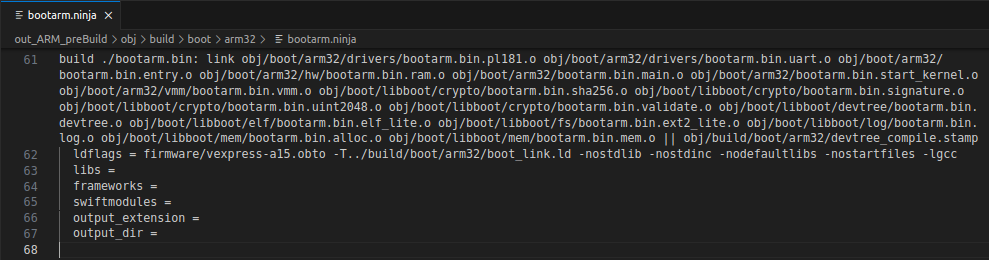
\includegraphics[scale=0.4]{compileLink_ARM.png}
		}
		\vspace*{0.3cm}
		\subfloat[\texttt{x86}]{
			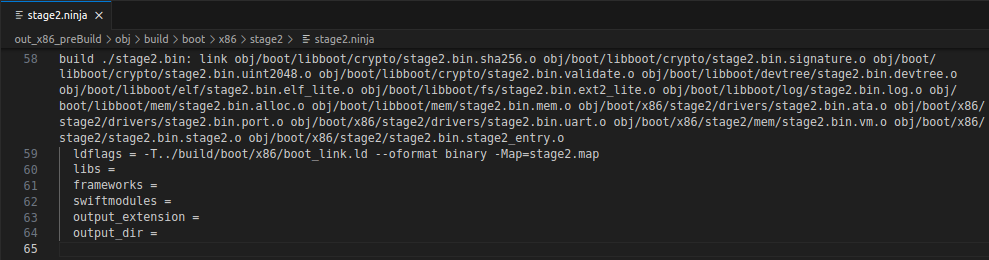
\includegraphics[scale=0.4]{compileLink_x86.png}
		}
		\caption{
			Instrucción de enlace de los archivos objeto generados del código fuente, similar a los archivos \texttt{Makefile} de los \textit{kernel} del curso.
			\label{fig:compileLink}
		}
	\end{figure}
	
	
	

\newpage
\subsection{Implementación del \textit{bootloader} \label{ssec:implBootloader}}
	Durante los temas vistos en el curso de Sistemas Operativos se vio que, 
	cuando se construye un sistema, una parte vital para el arranque es que el \textit{bootloader} otorgue control a dicho sistema (\autoref{fig:arranqueSO}), en el caso de \texttt{OpuntiaOS}, se tiene un manejo de la construcción del arranque con archivos \texttt{ninja}.
	\begin{figure}[ht]
		\centering
		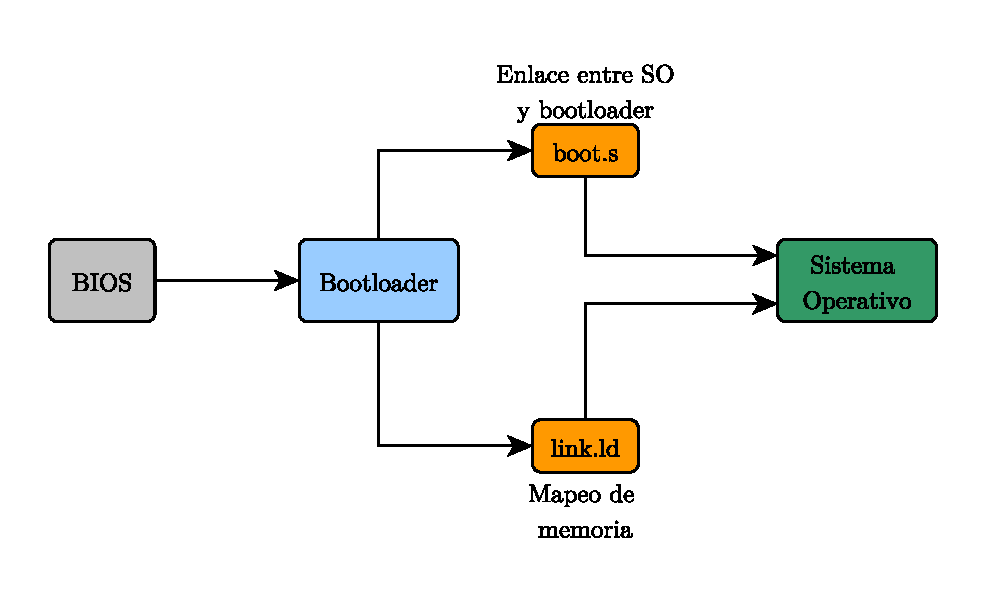
\includegraphics[scale=0.8]{arranqueSO.eps}
		\caption{
			Proceso de arranque de un sistema operativo.
			\label{fig:arranqueSO}
		}
	\end{figure}
	
	

	Lo primero de lo que es posible percatarse al analizar la implementación del \textit{bootloader} es que la estructura de carpetas y archivos es distinta para \texttt{ARM} y \texttt{x86}.
	\begin{figure}[ht]
		\centering
		\subfloat[\texttt{ARM} \label{sfig:implBloaderArm}]{
			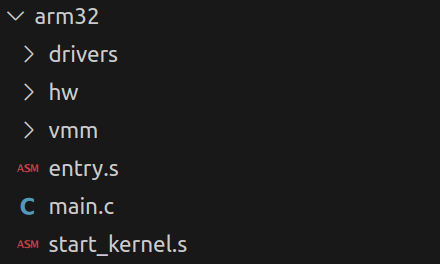
\includegraphics[scale=0.4]{estrucDir_ARM.png}
		}
		\hspace*{0.3cm}
		\subfloat[\texttt{x86} \label{sfig:implBloaderx86}]{
			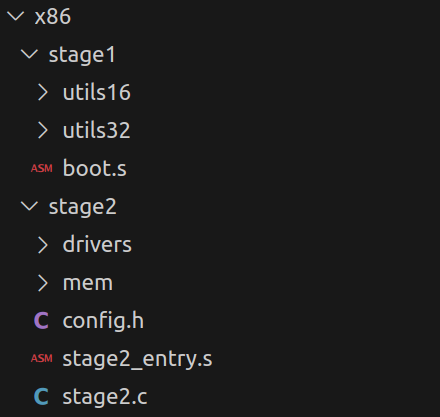
\includegraphics[scale=0.4]{estrucDir_x86.png}
		}
		\caption{
			Árbol de carpetas de implementación del \textit{bootloader}.
			\label{fig:implBootloader}
		}
	\end{figure}

	
	
	Por otra parte, se tiene el código de enlace (en el curso \texttt{link.ld}):
	\begin{itemize} \setlength\itemsep{0pt}
		\item \texttt{build/boot/x86/boot\_link.ld} para \texttt{x86},
		\item \texttt{build/boot/arm32/boot\_link.ld} para \texttt{ARM},
	\end{itemize}
	
	mismos que se llaman con ninja (ver \autoref{fig:compileLink}) y cabe mencionar que en el directorio \texttt{boot} se maneja la misma estructura que en la \autoref{fig:implBootloader}, pero solo con los archivos de construcción y el enlace.
	
	
	
	\subsubsection{En \texttt{x86}}
	En el caso de \texttt{OpuntiaOS} para \texttt{x86}, se manejan 2 archivos de etapa para el arranque del sistema en lugar de 1, es decir, no se generará el archivo \texttt{stage2\_eltorito}, si no que se generarán 2 archivos de carga de \textit{kernel}.
	\begin{figure}[ht]
		\centering
		\subfloat[Directorio \texttt{stage1} \label{sfig:x86Boot_stage1}]{
			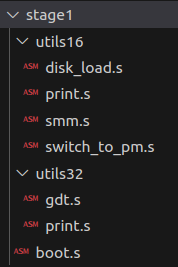
\includegraphics[scale=0.5]{x86_stage1_code.png}
		}
		\hspace*{1cm}
		\subfloat[Directorio \texttt{stage2} \label{sfig:x86Boot_stage2}]{
			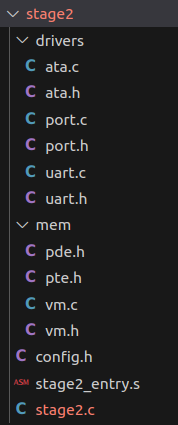
\includegraphics[scale=0.5]{x86_stage2_code.png}
		}
		\caption{
			Directorio de implementación del \textit{bootloader} para \texttt{x86}.
			\label{fig:x86Boot}
		}
	\end{figure}
	
	Como se aprecia en la \autoref{sfig:x86Boot_stage1}, la primera etapa de carga contiene solo código ensamblador, es to es porque \texttt{stage1} se carga desde la BIOS y es la encargado de realizar la primera carga del \textit{kernel}, se puede decir que el archivo más importante es \texttt{boot.s}, similar a los \textit{kernel} compilados en el curso.
	
	
	\clearpage
	Dentro del archivo \texttt{boot.s} se encuentra la carga del \textit{kernel} bajo instrucciones de 16 bits, que a su vez utiliza la carga del disco y mapeo de la memoria, y después la entrada a modo protegido, cuyas instrucciones deben considerarse de 32 bits y en este mismo tamaño de instrucciones se encuentra la definición de la GDT.
	\begin{figure}[ht]
		\centering
		\subfloat[Inclusión de utilidades para 16 y 32 bits. \label{sfig:x86_boots_include}]{
			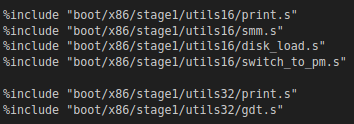
\includegraphics[scale=0.55]{x86_boots_include.png}
		}
		\vspace*{0.3cm}
		\subfloat[Código de 16 bits \label{sfig:x86_boots_16bits}]{
			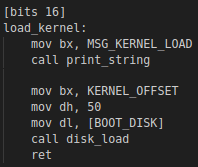
\includegraphics[scale=0.55]{x86_boots_16bits.png}
		}
		\hspace*{1cm}
		\subfloat[Código de 32 bits \label{sfig:x86_boots_32bits}]{
			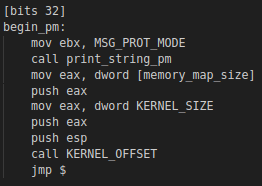
\includegraphics[scale=0.55]{x86_boots_32bits.png}
		}
		\caption{
			Código del archivo \texttt{boot.s} para la arquitectura \texttt{x86}.
			\label{fig:x86_boots}
		}
	\end{figure}

	Como se puede observar en la \autoref{fig:x86_boots}, se utilizan los registros de 16 bits además de los de 32, esto es debido a la retrocompatibilidad de la arquitectura \texttt{x86}.
	
	
	Por otro lado, en el \texttt{stage2} se tienen implementados lo siguientes controladores:
	\begin{itemize} \setlength\itemsep{0pt}
		\item Inicializador del disco de arranque (\texttt{ata.c} y \texttt{ata.h}).
		\item Lectura y escritura de puertos bajo 8, 16 y 32 bits (\texttt{port.c} y \texttt{port.h}).
		\item Inicialización y escritura de la interfaz UART (\texttt{uart.c} y \texttt{uart.h}).
	\end{itemize}
	
	
	
	Y también está la implementación del manejador de memoria:
	\begin{itemize} \setlength\itemsep{0pt}
		\item Definición de los descriptores de página (\texttt{pte.h}).
		\item Definición de los descriptores de tablas (\texttt{pde.h}).
		\item Memoria virtual del sistema utilizando paginación (\texttt{vm.c} y \texttt{vm.h}), y por lo tanto, los descriptores de tablas y de páginas de los 2 puntos anteriores.
	\end{itemize}

	
	
	Esta etapa es la que se encarga de cargar el \textit{kernel} a la memoria, esto se realiza preparando el disco de arranque por medio del archivo \texttt{stage2\_entry.s}.
	
	
	
	Esto lo hace inicializando la pila del procesador con ayuda del archivo enlazador para dar paso al \textit{kernel}, luego el encargado de realizar el proceso principal de la segunda etapa es \texttt{stage2.c}, que contiene el código para iniciar la memoria de arranque, preparar el disco y el sistema de archivos, validar el \textit{kernel} encontrado, cargar el \textit{kernel} a la memoria e iniciar la paginación de la memoria.

	
	
	
	\subsubsection{En \texttt{ARM}}
	En el caso de \texttt{OpuntiaOs} para \texttt{ARM} se debe entender cómo funciona el arranque de dicha arquitectura.
	
	
	
	\texttt{ARM} es una arquitectura que se utiliza para los SoC (Sistemas en Chip) y sigue un proceso de arranque similar al de una PC con \texttt{x86}, con la diferencia de que la información encesaria para arrancar no se carga desde un disco duro, si no desde una tarjeta \texttt{SD} y su \textit{bootloader} no es \texttt{GRUB}, si no que es \texttt{U-boot} \cite{vargas_risc}.

	
	
	Una de las principales diferencias a nivel de código es que la dirección de arranque de \textit{kernel} no comienza en la dirección \texttt{0x80000000} como en \texttt{x86}, si no que lo hace en la \texttt{0x00000000}.
	
	
	
	El \textit{bootloader} de \texttt{ARM} trabaja en 2 etapas, la primera que trabaja en modo supervisor, que se encarga de acceder a los recursos del sistema y poder ejecutar el \textit{kernel} del sistema, siendo también el modo donde se ejecuta el sistema operativo en sí; luego está la etapa de modo usuario, donde se restringe el acceso a \textit{hardware}, se ejecutan solo algunas instrucciones a nivel ensamblador y se tienen todas las aplicaciones que el usuario necesita y a las que puede acceder.
	
	
	
	Gracias al modo de arranque en modo supervisor de esta arquitectura, su código de arranque es más sencillo, no solo porque tiene un acceso más directo al \textit{hardware} en el mismo nivel donde trabaja el sistema operativo, si no que se basa en instrucciones \texttt{RISC}, lo cual baja complejidad al código utilizado para su manipulación.
	\begin{figure}[ht]
		\centering
		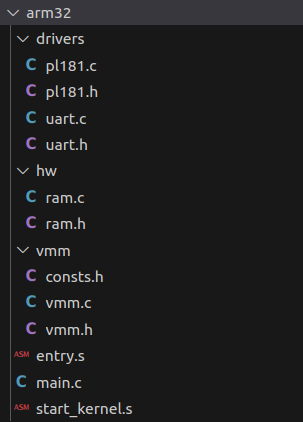
\includegraphics[scale=0.5]{arm_boot_code.png}
		\caption{
			Directorio de implementación del \textit{bootloader} para \texttt{ARM}.
			\label{fig:arm_boot_code}
		}
	\end{figure}
	
	\newpage
	
	En esta arquitectura las instrucciones son de 32 bits y los archivos principales del \textit{bootloader} son:
	\begin{itemize} \setlength\itemsep{0pt}
		\item \texttt{entry.s}: Contiene el código que se ejecuta en primer lugar cuando se enciende la máquina, se encarga de iniciar la pila y, como los diferentes sistemas en chip pueden tener uno o varios procesadores, se encarga de recorrer los id de cada procesador para iniciar cada pila adecuadamente .
		\item \texttt{start\_kernel.s}: Este código inicializa las estructuras de datos del \textit{kernel} y configura el sistema operativo, por medio de la llamada al archivo principal de configuración \texttt{main.c} luego de realizar esto, comienza la ejecución del \textit{kernel}.
	\end{itemize}
	\begin{figure}[ht]
		\centering
		\subfloat[]{
			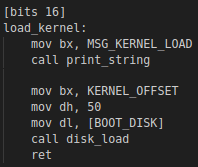
\includegraphics[scale=0.55]{x86_boots_16bits.png}
		}
		\hspace*{1cm}
		\subfloat[]{
			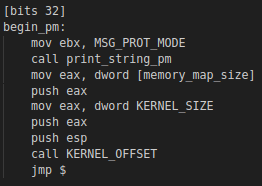
\includegraphics[scale=0.55]{x86_boots_32bits.png}
		}
		\caption{
			Código del archivo \texttt{start\_kernel.s} para la arquitectura \texttt{ARM}.
			\label{fig:arm_startkernels}
		}
	\end{figure}

	
	\clearpage
	Por otro lado, se tienen implementados los siguientes archivos:
	\begin{itemize} \setlength\itemsep{0pt}
		\item \textbf{Controladores}
		\begin{itemize} \setlength\itemsep{0pt}
			\item Mapeo y lectura de la tarjeta SD de donde se va a cargar el sistema operativo, debe su nombre a la celda 
			PL181\footnote{
				La tarjeta multimedia \texttt{PL180/181} es un periférico \texttt{ARM} para tarjetas multimedia (MMC) y tarjetas digitales seguras (SD) en formato de E/S, asignadas en memoria compatible con el bus periférico avanzado (APB) de \texttt{ARM} \cite{pl181}.
			}
			donde se introducen dichas tarjetas (\texttt{pl181.c} y \texttt{pl181.h}).
			
			\item Inicialización y lectura de la interfaz UART (\texttt{uart.c} y \texttt{uart.h}).
		\end{itemize}
	
		\item \textbf{Manejo de \textit{hardware}}
		\begin{itemize} \setlength\itemsep{0pt}
			\item Lector de tamaño de la memoria RAM instalada en el dispositivo (\texttt{ram.c} y \texttt{ram.h}).
		\end{itemize}
	
		\item \textbf{Manejo de memoria}
		\begin{itemize} \setlength\itemsep{0pt}
			\item Definición de constantes para el manejo de la memoria virtual (\texttt{consts.hh}).
			
			\item Memoria virtual del sistema utilizando paginación,para ello definiendo las estructuras para los descriptores de tablas y de páginas (\texttt{vmm.c} y \texttt{vmm.h}), utilizando las constantes definidas del punto anterior.
		\end{itemize}
	\end{itemize}

	
	\newpage
	La implementación del \textit{bootloader} de ambas arquitecturas utiliza, en común, los archivos del directorio \texttt{libboot}, que contiene las estructuras de datos y algunas implementaciones para hacer la validación del sistema (firma, seguridad, sistema de archivos \texttt{ext2}, etc.) y que éste arranque de forma correcta y segura.
	\begin{figure}[ht]
		\centering
		\subfloat[]{
			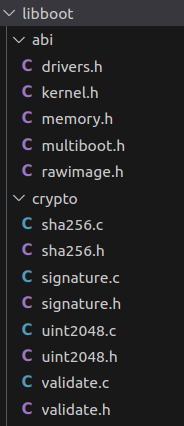
\includegraphics[scale=0.5]{libboot_p1.png}
		}
		\hspace*{1cm}
		\subfloat[]{
			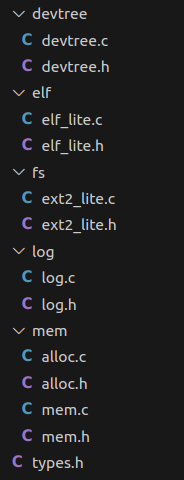
\includegraphics[scale=0.5]{libboot_p2.png}
		}
		\caption{
			Archivos del directorio \texttt{libboot}, común para las arquitecturas analizadas (\texttt{ARM} y \texttt{x86}).
			\label{fig:libboot}
		}
	\end{figure}

	
	
	Otro directorio que implementan en común las 2 arquitecturas es \texttt{libs}, que contiene, entre otras cosas, manejadores de memoria, definiciones para funcionamiento de la interfás gráfica y las definiciones de funciones para lenguaje \texttt{C}, tales como \texttt{malloc, execve, fork}, etc.
	\begin{figure}[ht]
		\centering
		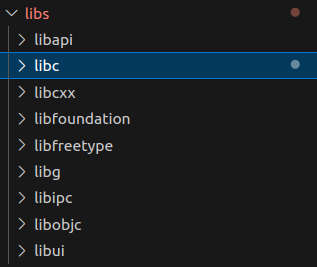
\includegraphics[scale=0.5]{libs.png}
		\caption{
			Directorio \texttt{libs}.
			\label{fig:libs}
		}
	\end{figure}
	

\newpage
\subsection{Comparativa \texttt{ARM} y \texttt{x86}}
	En principio, el \textit{bootloader} de ambas arquitecturas presenta similitudes en cuanto a las tareas básicas del sistema.
	
	
	
	Una similitud se encuentra en la manera en que funcionan, porque ambos se encargan de realizar las tareas básicas de arranque del sistema, como:
	\begin{itemize} \setlength\itemsep{0pt}
		\item \textbf{Inicialización del hardware}: Detectar y configurar la memoria, el CPU, los dispositivos de almacenamiento y otros componentes del sistema.
		
		\item \textbf{Carga del sistema operativo}: Buscar y cargar el \textit{kernel} del sistema operativo en la memoria.
		
		\item \textbf{Transferencia de control}: Transferir el control al \textit{kernel} del sistema operativo para que se inicie el sistema.
	\end{itemize}

	Y otro aspecto similar es la estructura que tienen, porque ambos tienen una fase de arranque temprano y una fase de arranque tardío.
	\begin{itemize} \setlength\itemsep{0pt}
		\item \textbf{Fase de arranque temprano}: Se ejecuta en \textbf{modo real} en \texttt{x86} y en \textbf{modo supervisor} en \texttt{ARM}. 
		
		
		
		En esta fase se hace una inicialización básica del \textit{hardware} y carga el \textit{kernel} del \textit{bootloader}.
		
		
		\item \textbf{Fase de arranque tardío}: Se ejecuta en \textbf{modo protegido} en \texttt{x86} y en \textbf{modo usuario} en \texttt{ARM}. 
		
		
		
		En esta fase se cargan los controladores adicionales, la configuración del sistema y la presentación de un menú de arranque.
	\end{itemize}
	
	
	
	Luego, de acuerdo con la información analizada en la \autoref{ssec:implBootloader}, es posible notar varias diferencias en la manera en que se arranca el sistema en las arquitecturas \texttt{ARM} y \texttt{x86}, en la \autoref{tab:bootldrCompArranque} se presenta una comparativa entre ellas.
	\begin{table}[ht]
		\centering
		\begin{tabular}{|
				>{\columncolor[HTML]{ECF4FF}}c |c|c|}
			\hline
			\multicolumn{1}{|l|}{\cellcolor[HTML]{000000}} & \cellcolor[HTML]{68CBD0}\textbf{x86} & \cellcolor[HTML]{68CBD0}\textbf{ARM}                                                    \\ \hline
			\textbf{Instrucciones}                         & Complejas, de 16 y 32 bits           & Reducidas, de 32 bits                                                                     \\ \hline
			\textbf{Modo de arranque}                      & En modo real                         & En modo supervisor                                                                      \\ \hline
			\textbf{Acceso a hardware}                     & Tiene acceso directo                 & \begin{tabular}[c]{@{}c@{}}Utiliza interfaces del \\ firmware del sistema\end{tabular} \\ \hline
			\textit{\textbf{Firmware}}                     & Utiliza BIOS                         & Utiliza U-Boot o UEFI                                                                   \\ \hline
			\textbf{Herramientas}                          & GRUB y LILO                          & U-Boot y UEFI                                                                           \\ \hline
		\end{tabular}
		\caption{
			Comparación del modo de arranque de \texttt{ARM} y \texttt{x86}.
			\label{tab:bootldrCompArranque}
		}
	\end{table}
	
	\newpage
	
	Durante el curso de sistemas operativos se abordo el tema del modo real y modo protegido de la arquitectura\texttt{x86}, siendo el primero cuando se tiene acceso directo a rutinas de la BIOS y el \textit{hardware} y el segundo cuando se restringe el acceso a privilegios del sistema usando GDT, IDT y memoria virtual por paginación.
	
	
	
	En \texttt{ARM} existen homólogos denominados ``modo supervisor'' y ``modo usuario'', que cumplen una función similar al modo real y protegido, respectivamente.
	
	
	Los modos supervisor y usuario de ARM se utilizan para:
	\begin{itemize} \setlength\itemsep{0pt}
		\item \textbf{Protección}
		\begin{itemize} \setlength\itemsep{0pt}
			\item \underline{Modo supervisor}: Permite el acceso a recursos sensibles como memoria, dispositivos de E/S e instrucciones privilegiadas. Se utiliza para ejecutar el \textit{kernel}, controladores de dispositivos y otras tareas críticas del sistema.
			
			\item \underline{Modo usuario}: Limita el acceso a recursos del sistema y solo permite ejecutar instrucciones no privilegiadas. Se usa para ejecutar aplicaciones de usuario, esto protege el sistema operativo y el \textit{hardware} de posibles errores o acciones maliciosas.
		\end{itemize}
	
		\item \textbf{Aislamiento}
		\begin{itemize} \setlength\itemsep{0pt}
			\item \underline{Modo supervisor}: Ofrece un entorno seguro para ejecutar el sistema operativo y las tareas críticas del sistema, sin interferencias de las aplicaciones de usuario.
			
			\item \underline{Modo usuario}: Proporciona un entorno aislado para ejecutar aplicaciones de usuario, evitando que puedan acceder a recursos del sistema que no necesitan.
		\end{itemize}
	
		\item \textbf{Rendimiento}
		\begin{itemize} \setlength\itemsep{0pt}
			\item \underline{Modo supervisor}: Permite un mayor rendimiento al ejecutar código privilegiado que necesita acceso directo al \textit{hardware}.
			
			\item \underline{Modo usuario}: Permite un uso más eficiente de la memoria al ejecutar código no privilegiado en un espacio de memoria separado.
		\end{itemize}
	\end{itemize}

	
	
	En consecuencia, es posible comparar la funcionalidad de los modos de arranque para ambas arquitecturas, lo cuál se muestra en la \autoref{tab:bootldrCompStage1} y \autoref{tab:bootldrCompStage2}.
	\begin{table}[ht]
		\centering
		\begin{tabular}{|
				>{\columncolor[HTML]{ECF4FF}}c |c|c|}
			\hline
			\multicolumn{1}{|l|}{\cellcolor[HTML]{000000}}                                 & \cellcolor[HTML]{68CBD0}\textbf{Modo real} & \cellcolor[HTML]{68CBD0}\textbf{Modo supervisor}                            \\ \hline
			\textbf{Nivel de privilegios}                                                  & Bajo                                       & Alto                                                                        \\ \hline
			\textbf{Acceso a memoria}                                                      & Segmentado                                 & Completo                                                                    \\ \hline
			\textbf{\begin{tabular}[c]{@{}c@{}}Acceso a \\ dispositivos E/S\end{tabular}}  & Limitado                                   & Completo                                                                    \\ \hline
			\textbf{\begin{tabular}[c]{@{}c@{}}Ejecución de \\ instrucciones\end{tabular}} & No privilegiadas                           & \begin{tabular}[c]{@{}c@{}}Privilegiadas y \\ no privilegiadas\end{tabular} \\ \hline
		\end{tabular}
		\caption{
			Comparación del modo real de \texttt{x86} y el modo supervisor de \texttt{ARM}.
			\label{tab:bootldrCompStage1}
		}
	\end{table}

	\begin{table}[ht]
		\centering
		\begin{tabular}{|
				>{\columncolor[HTML]{ECF4FF}}c |c|c|}
			\hline
			\multicolumn{1}{|l|}{\cellcolor[HTML]{000000}}                                 & \cellcolor[HTML]{68CBD0}\textbf{Modo protegido}                                & \cellcolor[HTML]{68CBD0}\textbf{Modo usuario}                                \\ \hline
			\textbf{Nivel de privilegios}                                                  & Alto                                                                           & Bajo                                                                         \\ \hline
			\textbf{Acceso a memoria}                                                      & \begin{tabular}[c]{@{}c@{}}Segmentado y \\ paginado\end{tabular}               & \begin{tabular}[c]{@{}c@{}}Limitado por \\ el segmento\end{tabular}          \\ \hline
			\textbf{\begin{tabular}[c]{@{}c@{}}Acceso a \\ dispositivos E/S\end{tabular}}  & \begin{tabular}[c]{@{}c@{}}Controlado por el \\ sistema operativo\end{tabular} & \begin{tabular}[c]{@{}c@{}}Limitado por el \\ sistema operativo\end{tabular} \\ \hline
			\textbf{\begin{tabular}[c]{@{}c@{}}Ejecución de \\ instrucciones\end{tabular}} & \begin{tabular}[c]{@{}c@{}}Privilegiadas y \\ no privilegiadas\end{tabular}    & \begin{tabular}[c]{@{}c@{}}No \\ privilegiadas\end{tabular}             \\ \hline
		\end{tabular}
		\caption{
			Comparación del modo protegido de \texttt{x86} y el modo usuario de \texttt{ARM}.
			\label{tab:bootldrCompStage2}
		}
	\end{table}
				
	\newpage
	
	En general, tanto los modos de \texttt{x86} como de \texttt{ARM} cumplen con las mismas funcione:
	\begin{itemize} \setlength\itemsep{0pt}
		\item Ambos pares de modos ofrecen diferentes niveles de acceso a los recursos del sistema.
		\item El modo con más privilegios se utiliza para ejecutar código crítico del sistema en espacio de \textit{kernel}, mientras que el menos privilegiado se utiliza para ejecutar aplicaciones en espacio de usuario.
	\end{itemize}	

	
	
	Sin embargo, basado en lo comparado en la \autoref{tab:bootldrCompStage1} y \autoref{tab:bootldrCompStage2}, así como en la \autoref{ssec:implBootloader}, se puede destacar lo siguiente:
	\begin{itemize} \setlength\itemsep{0pt}
		\item El modo supervisor es un modo de 32 bits, mientras que el modo real es un modo de 16 bits.
		
		\item El modo supervisor ofrece un mayor control sobre el \textit{hardware} y la memoria.
		
		\item El modo usuario ofrece un mayor aislamiento entre las aplicaciones.
		
		\item El modo protegido permite una gestión más eficiente de la memoria.
	\end{itemize}

	\newpage
	
	Finalmente se puede obtener una comparación entre el arranque del \textit{bootloader} de ambas arquitecturas.
	\begin{table}[ht]
		\centering
		\resizebox{\textwidth}{!}{ \begin{tabular}{|c|cc|}
			\hline
			\rowcolor[HTML]{68CBD0} 
			\multicolumn{1}{|l|}{\cellcolor[HTML]{000000}}                                & \multicolumn{1}{c|}{\cellcolor[HTML]{68CBD0}\textbf{x86}}                                                                                                                    & \textbf{ARM}                                                                                                                                                   \\ \hline
			\cellcolor[HTML]{ECF4FF}\textbf{Ubicación}                                    & \multicolumn{1}{c|}{\begin{tabular}[c]{@{}c@{}}MBR del disco \\ de arranque\end{tabular}}                                                                                    & \begin{tabular}[c]{@{}c@{}}Disco de arranque\\ (ej: tarjeta SD)\end{tabular}                                                                                   \\ \hline
			\cellcolor[HTML]{ECF4FF}\textbf{Modo de ejecución}                            & \multicolumn{1}{c|}{Modo real}                                                                                                                                               & Modo supervisor                                                                                                                                                \\ \hline
			\cellcolor[HTML]{ECF4FF}\textbf{Funciones}                                    & \multicolumn{1}{c|}{\begin{tabular}[c]{@{}c@{}}- Carga el \textit{kernel} del sistema operativo. \\ - Transfiere el control al \textit{kernel}. \\ - Ofrece un menú de arranque.\end{tabular}} & \begin{tabular}[c]{@{}c@{}}- Carga el \textit{kernel} del sistema operativo. \\ - Transfiere el control al \textit{kernel}. \\ - Puede ofrecer un menú de arranque.\end{tabular} \\ \hline
			\textbf{\begin{tabular}[c]{@{}c@{}}Diferencias más\\ relevantes\end{tabular}} & \multicolumn{1}{c|}{\begin{tabular}[c]{@{}c@{}}- Arranca en modo real. \\ - Código de 16 bits. \\ - Acceso directo al \textit{hardware}.\end{tabular}}                                & \begin{tabular}[c]{@{}c@{}}- Arranca en modo supervisor. \\ - Código de 32 bits (o 64 bits). \\ - Usa interfaces del \textit{firmware}.\end{tabular}                    \\ \hline
			\textbf{Similitudes}                                                          & \multicolumn{2}{c|}{\begin{tabular}[c]{@{}c@{}}- Carga el \textit{kernel} del sistema operativo. \\ - Transfiere el control al \textit{kernel}. \\ - Ofrece opciones de configuración.\end{tabular}}                                                                                                                                                            \\ \hline
			\cellcolor[HTML]{ECF4FF}\textbf{Ejemplos}                                     & \multicolumn{1}{c|}{GRUB, LILO}                                                                                                                                              & U-Boot, UEFI                                                                                                                                                   \\ \hline
		\end{tabular}}
		\caption{
			Comparación del funcionamiento del \textit{bootloader} de \texttt{ARM} y \texttt{x86}. 
			\label{tab:bootldrComparaGral}	
		}
	\end{table}
	

\clearpage
\subsection{Temas vistos en el curso de Sistemas Operativos}
	El código fuente del \textit{kernel} de \texttt{OpuntiaOS} se encuentra en el directorio \texttt{kernel} y está dividido en 2 directorios, \texttt{include} y \texttt{kernel}.
	
	
	
	Tal como muestra la \autoref{fig:kernel_code}, ambos directorios tienen, prácticamente, la misma estructura, pero el directorio \texttt{include} contiene archivo \texttt{.h} para definir las funciones y constantes necesarias para la compilación del \textit{kernel}, mientras que \texttt{kernel} contiene las implementaciones de estas cabeceras.
	\begin{figure}[ht]
		\centering
		\subfloat[Directorio \texttt{include} \label{sfig:kernel_code_include}]{
			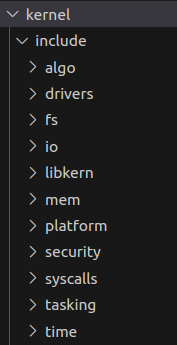
\includegraphics[scale=0.5]{kernel_code_include.png}
		}
		\hspace{3cm}
		\subfloat[Directorio \texttt{kernel} \label{sfig:kernel_code_kernel}]{
			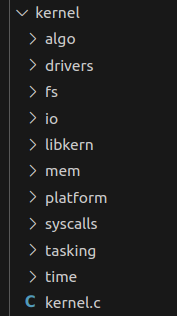
\includegraphics[scale=0.5]{kernel_code_kernel.png}
		}
		\caption{
			Directorio de implementación del \textit{kernel} de \texttt{OpuntiaOS}.
			\label{fig:kernel_code}
		}
	\end{figure}

	
	
	Una particularidad de esta estructura de carpetas es el directorio \texttt{platform}, el cual contiene las definiciones e implementaciones, respectivamente, que corresponden a cada una de las arquitecturas que soporta \texttt{OpuntiaOS}.
	
	
	
	A continuación se empatará el código visto en el curso con el contenido del código de \texttt{OpuntiaOS} siguiendo el orden del proyecto de James Molloy.
	
	
	
	\clearpage
	\subsubsection{Génesis}
		Archivos de Molloy: \texttt{boot.s, link.ld}.
		
		Para x86
		\begin{itemize} \setlength\itemsep{0pt}
			\item \texttt{build/boot/x86/boot\_link.ld}: El programa de carga se coloca en la dirección \texttt{0x1000}.
			\item \texttt{boot/x86/stage1/boot.s}: Carga del kernel.
			\item \texttt{boot/x86/stage2/stage2\_entry.s}: Inicialización de las estructuras del kernel.
		\end{itemize}
	
		NOTA: El archivo \texttt{boot/x86\_64/prekernel/mboot1.S} contiene una estructura mucho más similar al ensamblador proporcionado en el proyecto de Molloy, sin embargo el presente documento contempla la compilación en \texttt{x86} y no en \texttt{x86\_64}.
		
		
		Para ARM
		\begin{itemize} \setlength\itemsep{0pt}
			\item \texttt{build/boot/arm32/boot\_link.ld}: El programa de carga se coloca en la dirección \texttt{0x80010000}.
			\item \texttt{boot/arm32/entry.s}: Carga del kernel.
			\item \texttt{boot/arm32/start\_kernel.s}: Inicialización de las estructuras del kernel.
		\end{itemize}
		
		
		
	
	\subsubsection{La pantalla}
		En el código de Molloy se implementan los tipos de dato que se utilizan en todo el proyecto en el archivo \texttt{common.h} y \texttt{common.c}, en \texttt{OpuntiaOS} se usan:
		\begin{itemize} \setlength\itemsep{0pt}
			\item \texttt{boot/libboot/types.h}: Los tipos de dato que utiliza el \textit{bootloader}.
			
			\item \texttt{kernel/include/libkern/types.h}: Los tipos de dato que utiliza el código del \textit{kernel} para poder ser compilado.
			
			\item \texttt{libs/libc/include/sys/types.h}: Los tipos de dato que se utilizan como parte de la implementación, en lenguaje \texttt{C}, del sistema.
		\end{itemize}
	
		Estos archivos son utilizados por ambas arquitecturas.
	
		
		
		Luego, Molloy implementa el manejo de la pantalla con los archivos \texttt{monitor.h} y \texttt{monitor.c}; como \texttt{OpuntiaOS} es un sistema con ambiente gráfico, entonces se implementan los siguientes manejadores de pantalla:
		
		la pantalla tal como se vio en el curso, colocando la dirección de memoria de arranque de pantalla, pero se incluye el manejo de el ambiente gráfico y soporte de ventanas del sistema:
		\begin{itemize} \setlength\itemsep{0pt}
			\item \textbf{Inicialización y control}: Similar al proyecto en clase, se utiliza la pantalla con sus direcciones de memoria y manipulación de caracteres, se usan las definiciones en
			\texttt{kernel/include/drivers/debug/screen.h}\\
			y las implementaciones en 
			\texttt{kernel/kernel/drivers/debug/screen.c}.
			
			\item \textbf{Interfaz gráfica}: Se define el soporte para la interfaz gráfica del sistema en 
			\texttt{libs/libui/include/libui/Screen.h} y se utiliza en \\
			\texttt{libs/libui/src/Window.cpp}. \\
			Como puede notarse, esta implementación es en \texttt{C++}.
			
			
			\item \textbf{Ventanas del sistema}: Se define el manejo de ventanas en el archivo \texttt{userland/servers/window\_server/src/devices/Screen.h}, que se implementa en \texttt{userland/servers/window\_server/src/devices/Screen.cpp}, siendo desarrollado en \texttt{C++} y usándose en varios archivos dentro de\\ \texttt{userland/servers/window\_server/src/Components}.
		\end{itemize}
	
		Estos archivos son utilizados por ambas arquitecturas.
	
	
	
	
	
	\subsubsection{GDT e IDT}
		Archivos de Molloy: \texttt{gdt.s, interrupt.s, descriptor\_tables.h, descriptor\_tables.c, isr.h, isr.c}.
		
		Para x86:
		\begin{itemize} \setlength\itemsep{0pt}
			\item Ensambladores
			\begin{itemize} \setlength\itemsep{0pt}
				\item \texttt{boot/x86/stage1/utils32/gdt.s}
				\item \texttt{kernel/kernel/platform/x86/i386/interrupts/interrupts.s}
			\end{itemize}	
		
			\item Descriptor de la GDT
			\begin{itemize} \setlength\itemsep{0pt}
				\item \texttt{kernel/include/platform/x86/gdt.h}
				\item \texttt{kernel/kernel/platform/x86/gdt.c}
			\end{itemize}	
		
			\item Descriptor de la IDT
			\begin{itemize} \setlength\itemsep{0pt}
				\item \texttt{kernel/include/platform/x86/idt.h}
				\item \texttt{kernel/kernel/platform/x86/interrupts/idt.c}
			\end{itemize}
			
			\item Parte donde se inicia la GDT e IDT
			\begin{itemize} \setlength\itemsep{0pt}
				\item \texttt{kernel/include/platform/x86/init.h}
				\item \texttt{kernel/kernel/platform/x86/init.c}
			\end{itemize}	
			
			\item Manejador de IRQ
			\begin{itemize} \setlength\itemsep{0pt}
				\item \texttt{kernel/include/platform/x86/irq\_handler.h}
				\item \texttt{kernel/kernel/platform/x86/interrupts/irq\_handler.c}
			\end{itemize}	
			
			\item Rutinas de interrupciones (ISR)
			\begin{itemize} \setlength\itemsep{0pt}
				\item \texttt{kernel/include/platform/x86/isr\_handler.h}
				\item \texttt{kernel/kernel/platform/x86/interrupts/isr\_handler.c}
			\end{itemize}	
		\end{itemize}
	
		La arquitectura ARM no utiliza una GDT ni una IDT de la misma manera que lo hace la x86.
		
		%En la arquitectura x86, la GDT se utiliza para almacenar descripciones de segmentos de memoria y la IDT se utiliza para gestionar las interrupciones. Estos conceptos están relacionados con la gestión de memoria y la manipulación de interrupciones en la arquitectura x86.
		
		ARM utiliza un modelo de segmentación de memoria plano (\textit{Flat Memory Model}), lo que significa que no hay segmentos de memoria separados como en x86. En lugar de la IDT, ARM utiliza vectores de interrupción y excepción.
		
		
	
		Para ARM:
		\begin{itemize} \setlength\itemsep{0pt}
			\item Ensambladores
			\begin{itemize} \setlength\itemsep{0pt}
				\item \texttt{kernel/kernel/platform/arm32/interrupts/interrupts.s}
			\end{itemize}
		
			\item Descriptor de la tabla genérica de interrupciones
			\begin{itemize} \setlength\itemsep{0pt}
				\item \texttt{kernel/include/drivers/irq/arm/gicv2.h}
				\item \texttt{kernel/kernel/drivers/irq/arm/gicv2.c}
			\end{itemize}
		
			\item Configuración de interrupciones y excepciones
			\begin{itemize} \setlength\itemsep{0pt}
				\item \texttt{kernel/include/platform/arm32/interrupts.h}
				\item \texttt{kernel/kernel/platform/arm32/interrupts/handlers.c}
			\end{itemize}
		
			\item Parte del código donde se inicia el controlador genérico de interrupciones (GIC) y las interrupciones.
			\begin{itemize} \setlength\itemsep{0pt}
				\item \texttt{kernel/include/platform/arm32/init.h}
				\item \texttt{kernel/kernel/platform/arm32/init.c}
			\end{itemize}	
		\end{itemize}
	
	
		
	
	
	\subsubsection{IRQ y PIT}
		Archivos de Molloy: \texttt{timer.h, timer.c}.
		
		La PIT)es un componente se utiliza para generar interrupciones periódicas, como las interrupciones del sistema operativo que pueden ser usadas para mantener el tiempo del sistema, gestionar tareas programadas, etc.
		
		En la arquitectura ARM no hay un PIT estándar, por otro lado, pueden usar temporizadores o contadores específicos que son parte del diseño del sistema embebido o del SoC, que pueden variar entre diferentes dispositivos.
		
		Para ambas arquitecturas se implementa un Administrador principal de \textit{ticks}:\\
		\texttt{kernel/include/time/time\_manager.h} \\
		\texttt{kernel/kernel/time/time\_manager.c}
		
		Para x86
		\begin{itemize} \setlength\itemsep{0pt}
			\item \texttt{kernel/include/drivers/timer/x86/pit.h}
			\item \texttt{kernel/kernel/drivers/timer/x86/pit.c}
			
		\end{itemize}
	
		Para ARM:
		En el caso de OpuntiaOS, se implementa un temporizador enfocado en el temporizador SP804
		\begin{itemize} \setlength\itemsep{0pt}
			\item \texttt{kernel/kernel/drivers/timer/arm/sp804.c}
			\item \texttt{kernel/include/drivers/timer/arm/sp804.h}
		\end{itemize}
		
	
		

	
	\subsubsection{Paginación}
		Archivos de Molloy: \texttt{paging.h, paging.c, kheap.h, kheap.c}.
		
		
		Se usa el \textit{heap} para los archivos en \texttt{kernel/kernel/io}.
		
		\begin{itemize} \setlength\itemsep{0pt}
			\item Definición del \textit{heap} y su control
			\begin{itemize} \setlength\itemsep{0pt}
				\item \texttt{kernel/include/mem/kmalloc.h}
				\item \texttt{kernel/kernel/mem/kmalloc.c}
			\end{itemize}
			
			\item Gestión de la memoria virtual
			\begin{itemize} \setlength\itemsep{0pt}
				\item \texttt{kernel/include/mem/vmm.h}
				\item \texttt{kernel/kernel/mem/vmm.c}
			\end{itemize}
			
		\end{itemize}
	
		Se utiliza el mismo manejo de memoria para ambas arquitecturas.
		
	
	
	
	\subsubsection{VFS}
		Archivos de Molloy: \texttt{fs.h, fs.c, initrd.h, initrd.c, multiboot.h}.
		
		Se maneja el mismo sistema de archivos para ambas arquitecturas, en este caso, \texttt{ext2}
		\begin{itemize} \setlength\itemsep{0pt}
			\item Creación del \textit{ramdisk}
			\begin{itemize} \setlength\itemsep{0pt}
				\item \texttt{kernel/include/drivers/storage/ramdisk.h}
				\item \texttt{kernel/kernel/drivers/storage/ramdisk.c}
			\end{itemize}
		
			\item Definición del sistema de archivos virtual
			\begin{itemize} \setlength\itemsep{0pt}
				\item \texttt{kernel/kernel/fs/vfs.h}
				\item \texttt{kernel/include/fs/vfs.c}
			\end{itemize}
		
			\item Definición del sistema de archivos \texttt{ext2}, aquí se encuentra definido el superbloque.
			\begin{itemize} \setlength\itemsep{0pt}
				\item \texttt{kernel/include/fs/ext2/ext2.h}
				\item \texttt{kernel/kernel/fs/ext2/ext2.c}
			\end{itemize}
		\end{itemize}
		
	
	\subsubsection{Multitarea}
		Archivos de Molloy: \texttt{process.s, task.h, task.c}.
		
		En ambas arquitecturas se tiene la implementación común de tareas:
		\begin{itemize} \setlength\itemsep{0pt}
			\item \texttt{kernel/include/tasking/tasking.h}
			\item \texttt{kernel/kernel/tasking/tasking.c}
		\end{itemize}
	
		Sin embargo, cada una tiene su propia implementación particular.
		
		Para x86:
		\begin{itemize} \setlength\itemsep{0pt}
			\item implementación del TSS
			\begin{itemize} \setlength\itemsep{0pt}
				\item \texttt{kernel/include/platform/x86/tasking/tss.h}
				\item \texttt{kernel/kernel/platform/x86/tasking/tss.c}
			\end{itemize}
		\end{itemize}
		
		Para ARM:\\
		La implementación se divide en varios archivos \texttt{.c} y ensambladores, debido a que no se realiza de la misma manera que en \texttt{x86}, se encuentra en los archivos dentro de
		\texttt{kernel/kernel/platform/arm32/tasking}
		
		La implementación se realiza de esa manera porque el manejo de multitarea para ambas arquitecturas es diferente:
		\begin{itemize} \setlength\itemsep{0pt}
			\item \textbf{Interrupciones y Excepciones}: En \texttt{x86} la interrupción de temporizador (\textit{timer interrupt}) es crucial para implementar programación de tiempo compartido, mientras que en \texttt{ARM} define modos de operación (usuario, supervisor y otros) que se utilizan para gestionar niveles de privilegio.
			
			\item \textbf{Cambios de Contexto}: En \texttt{x86} el SO mantiene un contexto de registro y estado para cada tarea, luego cuando se produce una interrupción de temporizador solicitud de cambio, se guarda el contexto actual y se carga el contexto de la nueva tarea.
			
			Por otro lado, en \texttt{ARM} se mantiene un contexto de registro y estado para cada tarea en el espacio de memoria específico de cada tarea, luego cambiar entre tareas implica guardar y restaurar el contexto relevante.
			
			\item \textbf{Despacho de Tareas}: En \texttt{x86} se gestionan las prioridades de las tareas y se asigna tiempo de procesador según las políticas de planificación del SO, mientras que en \texttt{ARM} tanto la asignación de tiempo de procesador como la gestión de prioridades son parte de la lógica del planificador.
		\end{itemize}
	
	
	\subsubsection{Modo usuario}
		Archivos de Molloy: \texttt{syscall.h, syscall.c}.
		
		En el caso de \texttt{OpuntiaOS}, las llamadas al sistema se definen por medio del archivo \texttt{}, a manera de tabla de llamadas al sistema (como el \textit{kernel} de Linux).
		
		Luego se tienen los siguientes archivos relevantes:
		\begin{itemize} \setlength\itemsep{0pt}
			\item \texttt{kernel/include/libkern/bits/syscalls.h}: Definición del número de llamada al sistema para cada arquitectura.
			
			\item \texttt{kernel/include/syscalls/handlers.h}: Definición de las macros de funciones para implementar las llamadas y nombres de dichas funciones.
			
			\begin{itemize} \setlength\itemsep{0pt}
				\item \texttt{kernel/kernel/syscalls/handler.c}: Enlace del número de llamada con su macro de implementación, similar al archivo \texttt{.tbl} del \textit{kernel} de Linux.
			\end{itemize}
		\end{itemize}
	
		Esto es muy similar a cómo se compone el \textit{kernel} de Linux, lo cual tiene sentido porque \texttt{OpuntiaOS} es similar a Linux.
		
	
	
	
\clearpage
\subsection{Estructuras de datos más relevantes del sistema}
	\subsubsection{Administrador de procesos}
		Una de las estructuras más relevantes de Linux es el \texttt{task\_struct}, que define un proceso en el sistema, en el caso de \texttt{OpuntiaOS} se tiene la estructura \texttt{proc} (ver \autoref{prog:struct_proc}).
		
		El sistema también da soporte para hilos, implementando apuntadores a un proceso en específico (\autoref{prog:struct_thread}) y gracias a una lista doblemente enlazada.
		
		También se definen las llamadas a señales del sistema desde el espacio de usuario (ver \autoref{prog:struct_signals}).
		
		
		
		
	\subsubsection{Planificador}
		Otra estructura importante es \texttt{runqueue}, que utiliza una lista enlazada para poder crear hilos de ejecución y apuntadores a los procesos padre e hijo (o maestro y esclavo) que puedan crearse (ver \autoref{prog:struct_runqueue}).
		
		También se implementa el \textit{trapframe}, que almacena un conjunto de registros que guardados durante alguna excepción en la ejecución. Con ésta estructura es posible regresar a la ejecución cuando se maneja una excepción o una interrupción. El \textit{trapframe} es diferente para cada arquitectura (ver \autoref{prog:struct_trapframe_x86} y \autoref{prog:struct_trapframe_ARM})
		
		Por otro lado, el contexto es un conjunto de registros guardados por el destinatario, que representa el estado de la tarea antes de que otra la reemplazara (cambio de contexto). El \textit{context} es diferente para cada arquitectura (ver \autoref{prog:struct_context_x86} y \autoref{prog:struct_context_ARM}).
		
	
	
	\subsubsection{Administrador de memoria}
		Primeramente se tieneel ampeo de tablas, donde se almacenan las direcciones virtuales de los procesos a las direcciones físicas correspondientes en la memoria RAM (ver \autoref{prog:struct_mapentry}).
		
		La memoria utiliza una zona determinada dentro del sistema, esa zona está definida en la estructura dentro del \autoref{prog:struct_memzone}.
		
		Igualmente se tienen estructuradas las operaciones que son posibles en la memoria (ver \autoref{prog:struct_memop}).
		
		También se encuentra el espacio virtual de direcciones, que representa un área contigua de memoria virtual dentro del espacio de direcciones de un proceso. Cada región de memoria se gestiona mediante alguna estructura vm\_address\_space. (ver \autoref{prog:struct_memvspace}). Usa el algoritmo de arreglo dinámico.
		
		Como \texttt{OpuntiaOS} utiliza memoria paginada, cuenta con su tabla de páginas  (ver \autoref{prog:struct_mempaget}).
		
		
		
	\subsubsection{Sistema de archivos}
		La descripción de archivos es fundamental porque todo, en un sistema basado en Linux, se representa como un archivo. Las estructuras principales para esto, se muestran en el \autoref{prog:struct_files}.
		
		Otro aspecto fundamental es el superbloque i los i-nodos del sistema, para tener control e información de los archivos, esto se observa en el \autoref{prog:struct_ext2}.
		
		
		
	
	\subsubsection{Controladores de dispositivos}
		La definición de un dispositivo y los periféricos que pudiera estar utilizando se encuentra en la  \autoref{prog:struct_device}.
		
		Esta estructura se usa para definir un árbol de dispositivos del sistema, para controlar esto se utiliza una estructura diferente (ver \autoref{prog:struct_devtree}.
		
	
	

	
	